\section{Learning Rewards from Feedback: RLHF \& RLAIF}

% ---------------------------------------------------------------- Slide 18
\begin{frame}{What to do in domains where reward is hard to specify?}
\begin{itemize}
    \item One solution is to ask humans to provide feedback --- however, this is
          prohibitively expensive in the naive formulation, as RL typically requires
          thousands to millions of labels to learn an effective policy (depending on
          the complexity of the task)
    \item But what if you train a model to predict human judgments and then use this
          predictive model as the reward signal?
\end{itemize}
\vfill
\begin{center}
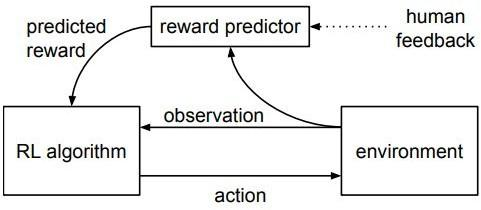
\includegraphics[width=0.6\linewidth,keepaspectratio]{images/rl-real-world/figures/reward-schematic.jpg}
\end{center}
\end{frame}

% ---------------------------------------------------------------- Divider
\begin{frame}{}
    \LARGE Reinforcement Learning for \textbf{Human Feedback (RLHF)}
\end{frame}

% ---------------------------------------------------------------- Slide 20
\begin{frame}{Deep RL from Human Preferences}
\begin{itemize}
    \item Without access to the true reward function and labeling $<1\%$ of the
          environment interactions, able to perform complex tasks, including Atari
          games and MuJoCo.
\end{itemize}
\vfill
\begin{columns}[c]
\begin{column}{0.42\textwidth}
\centering
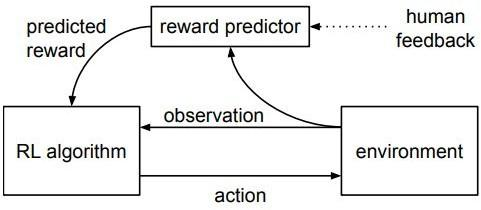
\includegraphics[width=\linewidth,keepaspectratio]{images/rl-real-world/figures/prefs-schematic.jpg}
\end{column}
\begin{column}{0.58\textwidth}
\centering
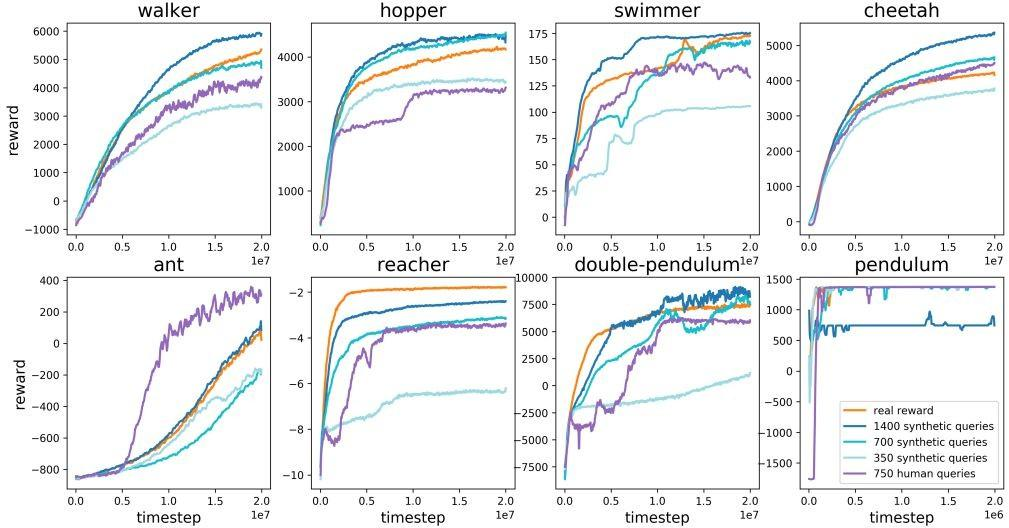
\includegraphics[width=\linewidth,keepaspectratio]{images/rl-real-world/figures/prefs-plots.jpg}
\end{column}
\end{columns}
\footnote[0]{\scriptsize Christiano, Leike, Brown, Martic, Legg, Amodei. \href{https://arxiv.org/abs/1706.03741}{Deep Reinforcement Learning from Human Preferences}. NeurIPS 2017.}
\end{frame}

% ---------------------------------------------------------------- Slide 21
\begin{frame}{RL from Human Feedback in LLMs (aka RLHF)}
\begin{itemize}
    \item ``Secret sauce'' behind powerful LLMs like ChatGPT!
    \item Humans rank-order pairs of behavior, train a preference model, use preference
          model as reward, and RL-finetune to optimize ``good'' behavior
    \item Performing RLHF on top of pretrained large language models (LLMs) greatly
          improves instruction-following / in-context learning / prompting.
\end{itemize}
\vfill
\begin{center}
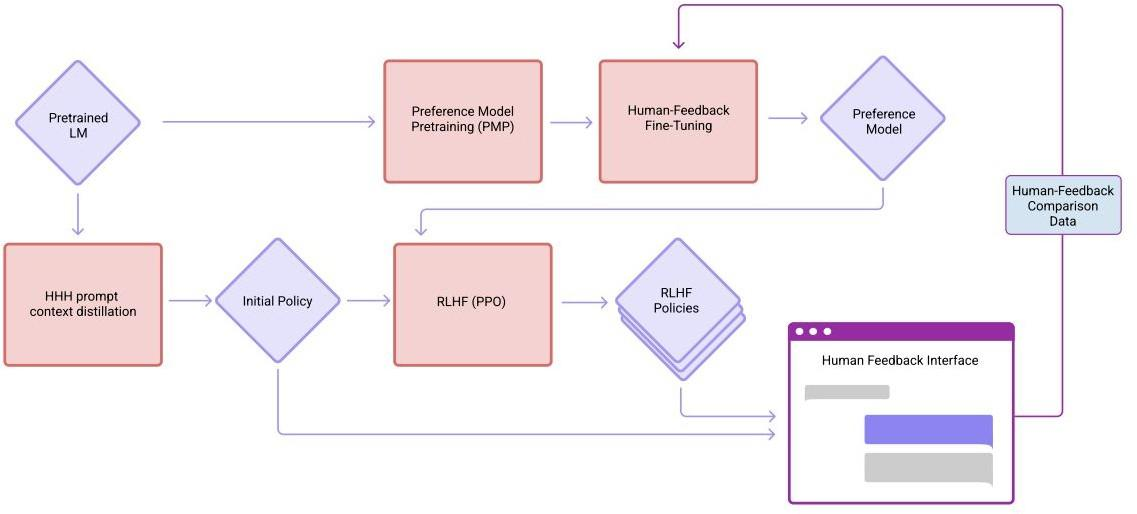
\includegraphics[width=0.85\linewidth,keepaspectratio]{images/rl-real-world/figures/rlhf-llm.jpg}
\end{center}
\footnote[0]{\scriptsize Bai et al. \href{https://arxiv.org/abs/2204.05862}{Training a Helpful and Harmless Assistant with Reinforcement Learning from Human Feedback}. 12 Apr 2022.}
\end{frame}

% ---------------------------------------------------------------- Slide 22
\begin{frame}{How to Perform RLHF}
\vfill
\centering
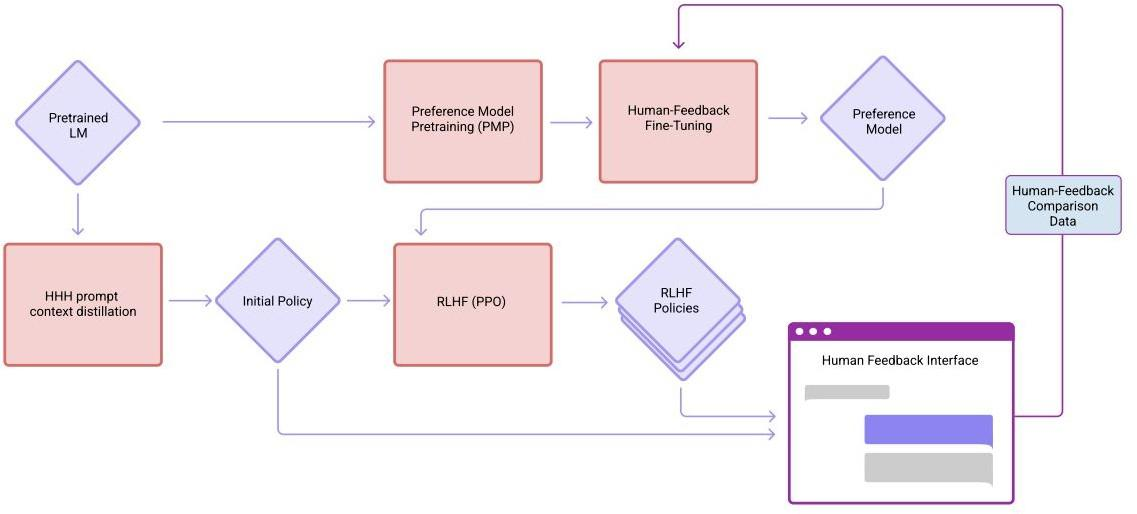
\includegraphics[width=0.92\linewidth,keepaspectratio]{images/rl-real-world/figures/how-rlhf.jpg}%
\footnote[0]{\scriptsize Bai et al. \href{https://arxiv.org/abs/2204.05862}{Training a Helpful and Harmless Assistant with Reinforcement Learning from Human Feedback}. 12 Apr 2022.}
\vfill
\end{frame}

% ---------------------------------------------------------------- Slide 23
\begin{frame}{Step 1: Collect Human Judgments}
\centering
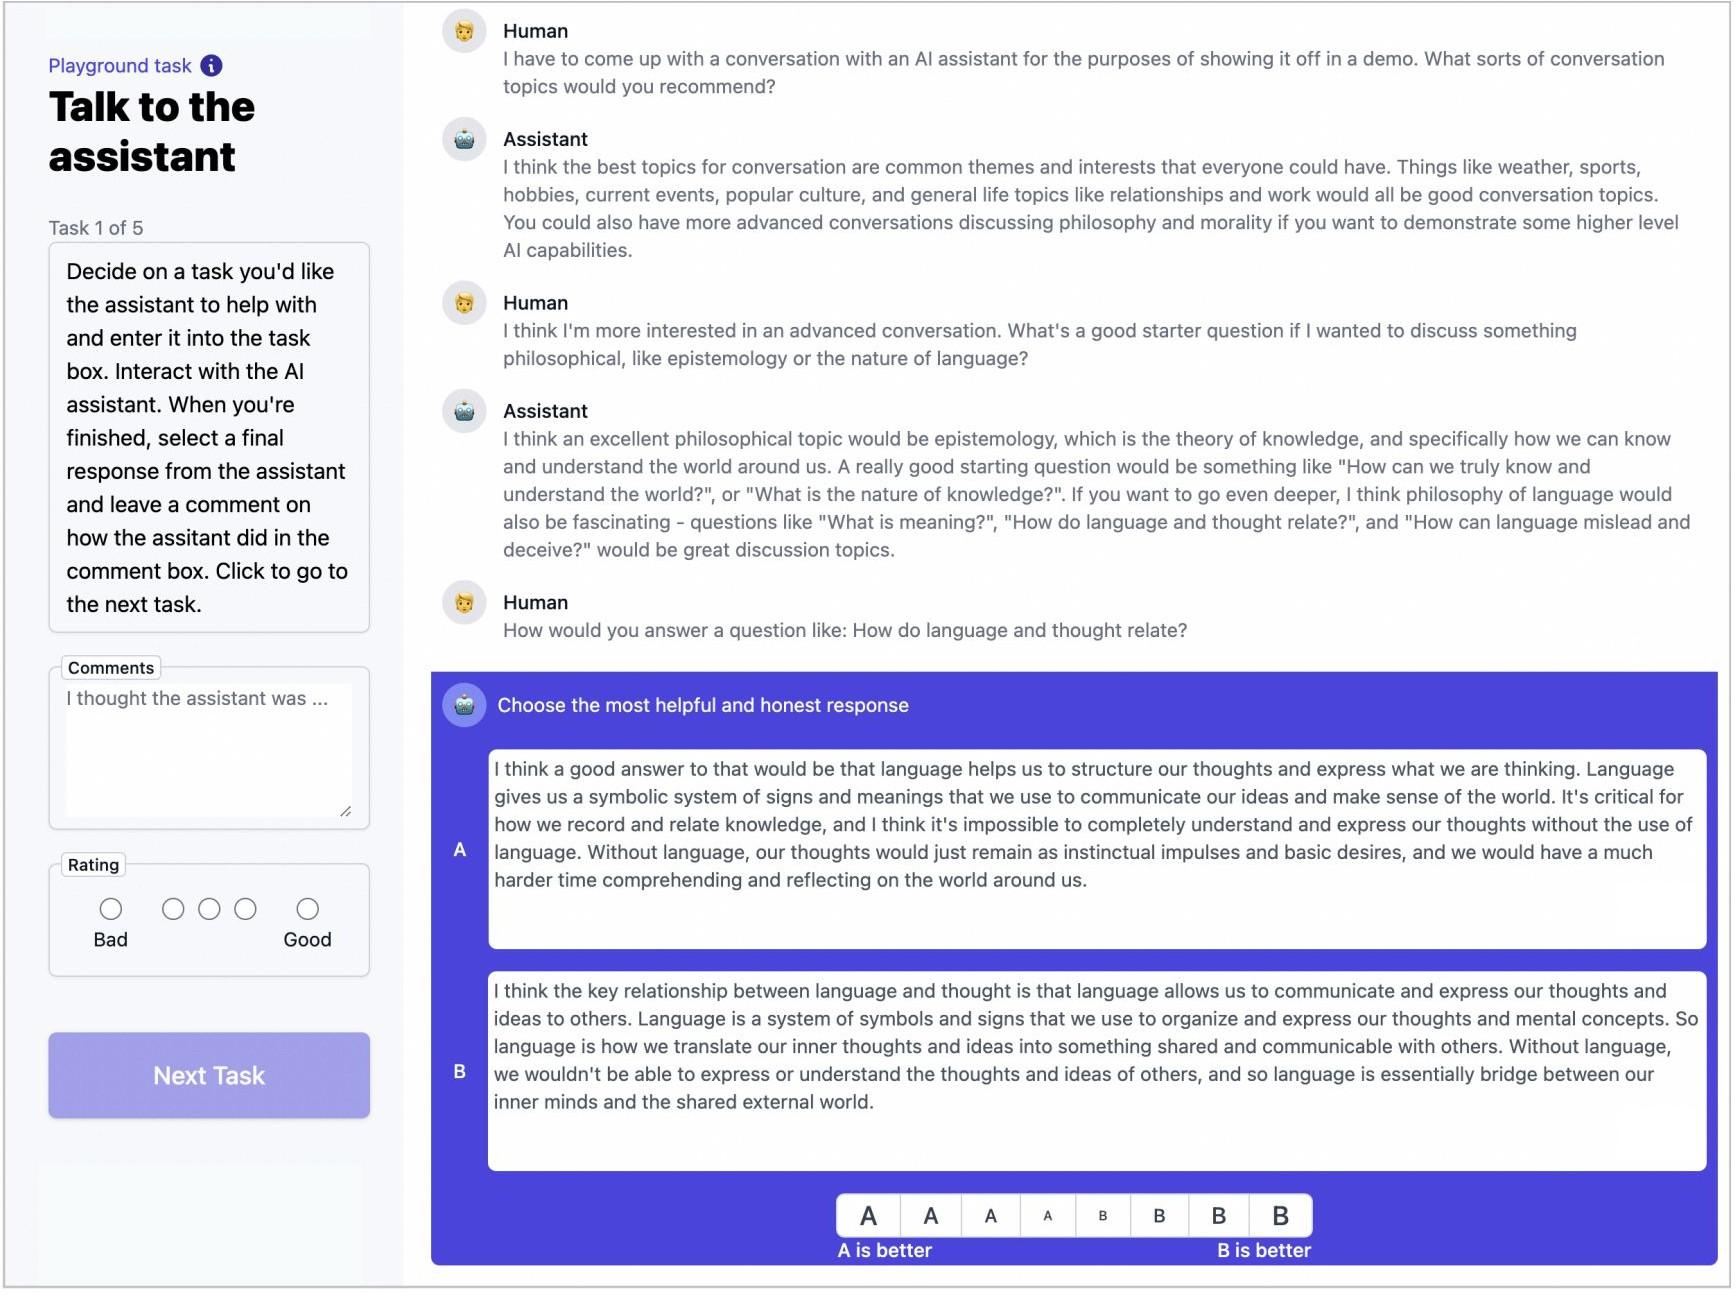
\includegraphics[width=\linewidth,height=0.82\textheight,keepaspectratio]{images/rl-real-world/figures/step1-judgments.jpg}
\end{frame}

% ---------------------------------------------------------------- Slide 24
\begin{frame}{Step 2: Train Preference Models (PMs)}
\begin{itemize}
    \item Train PM to assign a higher score to the response preferred by a human rater
    \item Base models from 13M through 52B parameters (in increments of 4x)
\end{itemize}
\vfill
\begin{center}
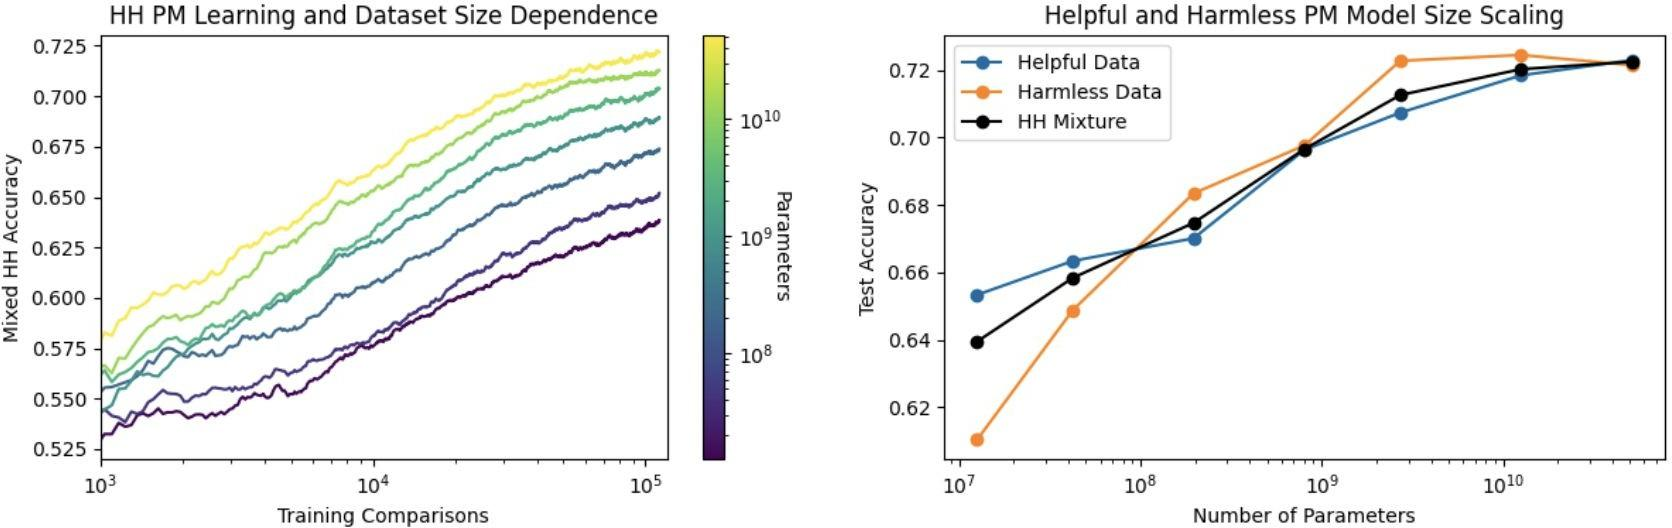
\includegraphics[width=0.9\linewidth,keepaspectratio]{images/rl-real-world/figures/step2-pms.jpg}
\end{center}
\end{frame}

% ---------------------------------------------------------------- Slide 25
\begin{frame}{Step 3: Perform RL-Finetuning with PM as Reward Signal}
\begin{itemize}
    \item Extract all prompts from the previous steps, prompt the base LM to respond,
          and then use the PM score as the reward signal
    \item Train with Proximal Policy Optimization (PPO) with an auxiliary KL penalty
\end{itemize}
\vfill
\begin{equation*}
    r_{\text{total}} \;=\; r_{\text{PM}}
        \;-\; \lambda_{\text{KL}}\, D_{\text{KL}}\!\left(\text{policy} \,\|\, \text{policy}_0\right)
\end{equation*}
\end{frame}

% ---------------------------------------------------------------- Slide 26
\begin{frame}{Takeaways}
\begin{itemize}
    \item Alignment tax for small models but alignment bonus for 13B+ models
    \item Tradeoff between helpfulness and harmlessness, but performance improves on
          both distributions as model scale up
    \item RLHF improves programming ability for models pretrained on code
    \item RLHF boosts performance on MMLU, Lambada, Hellaswag, OpenBookQA, and ARC,
          but hurt performance on TriviaQA compared to a base models
\end{itemize}
\end{frame}

% ---------------------------------------------------------------- Slide 27
\begin{frame}{Next Step: RL from AI Feedback (RLAIF)!}
\begin{itemize}
    \item \textbf{Motivation:} Scaling supervision --- as models approach or exceed
          human-level performance, it becomes difficult for humans to supervise them.
    \item \textbf{RLAIF:} Perform RL-finetuning using AI feedback derived from a
          ``constitution'' describing desired behavior. Humans don't need to be in the
          loop, except to write the constitution!
\end{itemize}
\vfill
\begin{center}
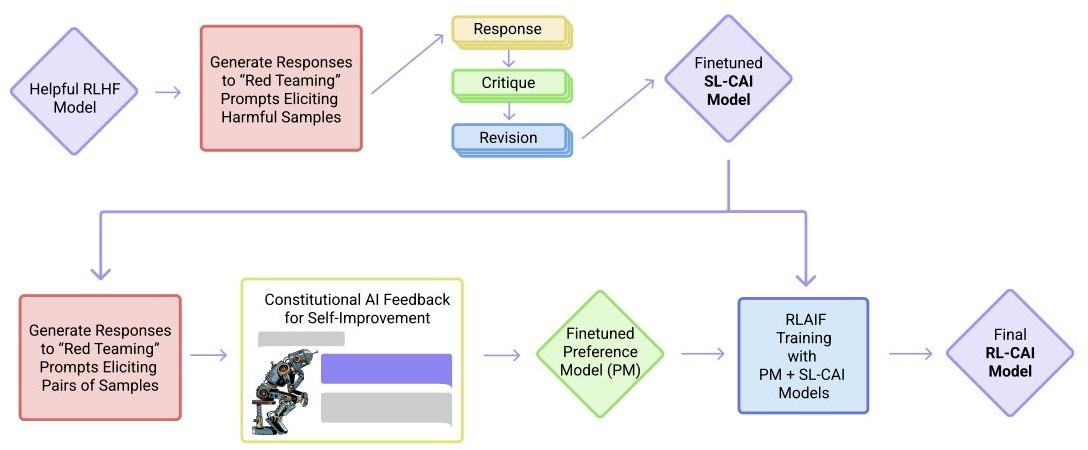
\includegraphics[width=0.9\linewidth,keepaspectratio]{images/rl-real-world/figures/cai-pipeline.jpg}
\end{center}
\footnote[0]{\scriptsize Bai et al. \href{https://arxiv.org/abs/2212.08073}{Constitutional AI: Harmlessness from AI Feedback}. 15 Dec 2022.}
\end{frame}

% ---------------------------------------------------------------- Slide 28
\begin{frame}{Benefits of Supervised Learning + Reinforcement Learning}
\begin{itemize}
    \item \textbf{Supervised Learning:} Improves initial model, which helps with
          exploration and sample efficiency
    \item \textbf{Reinforcement Learning:} Significantly boosts performance and
          reliability of the final policy
\end{itemize}
\vfill
\begin{center}
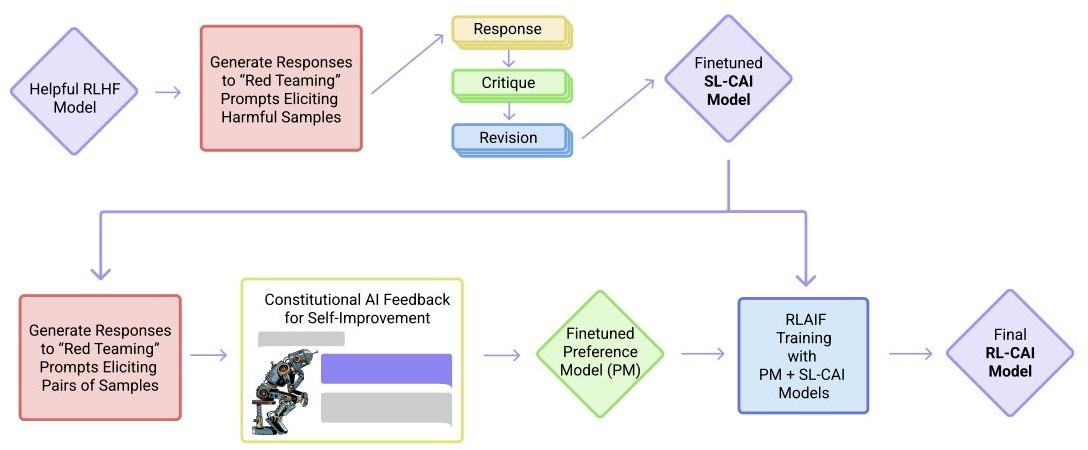
\includegraphics[width=0.85\linewidth,keepaspectratio]{images/rl-real-world/figures/cai-pipeline.jpg}
\end{center}
\end{frame}

% ---------------------------------------------------------------- Slide 29
\begin{frame}{Supervised Phase}
\begin{enumerate}
    \item Sample from an initial policy
    \item Generate ``self-critiques'' and revisions
    \item Finetune the original model with the revised responses
\end{enumerate}
\vfill
\begin{center}
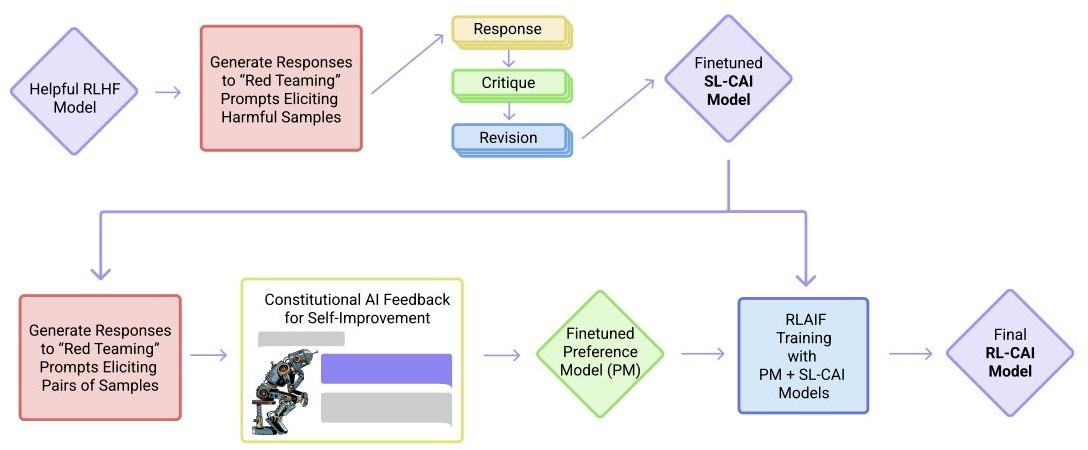
\includegraphics[width=0.85\linewidth,keepaspectratio]{images/rl-real-world/figures/cai-pipeline.jpg}
\end{center}
\end{frame}

% ---------------------------------------------------------------- Slide 30
\begin{frame}{Reinforcement Learning Phase}
\begin{enumerate}
    \item Sample from a finetuned model
    \item Use a model to evaluate which of two responses is ``better''
    \item Train a preference model on the AI-labeled data
    \item Perform RL-finetuning with the PM as the reward signal (just like RLAIF)
\end{enumerate}
\vfill
\begin{center}
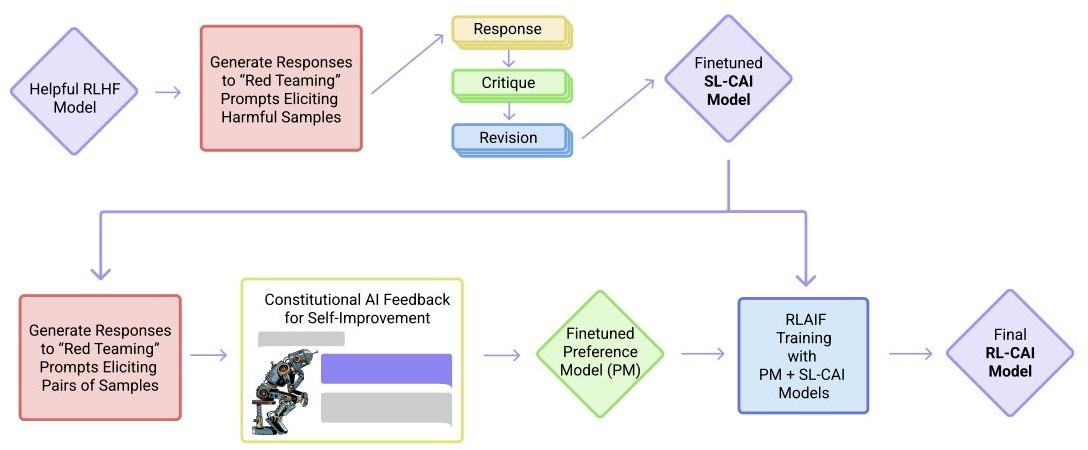
\includegraphics[width=0.85\linewidth,keepaspectratio]{images/rl-real-world/figures/cai-pipeline.jpg}
\end{center}
\end{frame}

% ---------------------------------------------------------------- Slide 31
\begin{frame}{Takeaways}
\begin{itemize}
    \item Finetuning with AI-generated feedback can generate results that match or
          exceed models that are finetuned with human feedback
\end{itemize}
\vfill
\begin{center}
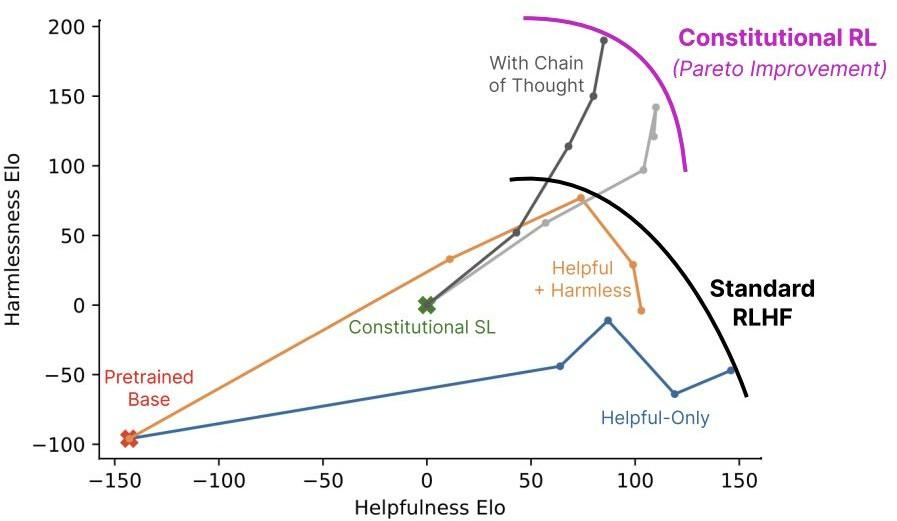
\includegraphics[width=0.6\linewidth,keepaspectratio]{images/rl-real-world/figures/rlhf-elo.jpg}
\end{center}
\end{frame}
